%\newpage
%================================================================
\section{Results and Discussion}\label{sec:Results}
%================================================================

%----------------------------------------------------------------
\subsection{Quantum Dot}
%----------------------------------------------------------------

We start with the simplest system of a single one-dimensional quantum dot, i.e., a system without repulsive interactions, in order to both validate the implementation and compare different settings for the training of the RBM. As mentioned in \autoref{sec:systems}, the exact ground state energy for this system is $1/2$ a.u. Throughout this study, the common variance of the Gaussian-binary RBM's visible layer is set to unity, the number of variational energy samples are held fixed at $2^{18}$ samples and in gradient descent optimization we use the ADAM algorithm.

%----------------------------------------------------------------
\subsubsection*{The Effect of the Learning Rate}
%----------------------------------------------------------------

\autoref{fig:train_iter_lr_batch1000} shows the effect of the learning rate $\eta$ with different numbers of training iterations. The training, or update of parameters, are done in batches of 1000 iterations, meaning that the x-axis tick labels correspond to the number of updates during training. Each point is the average of 8 Markov chains, each with expectation value of the energy, $\langle E \rangle$, the sampling error, $\sigma_b$, found via the blocking method, and the variance $\mathrm{Var}(E)$. In the figure, we show both results obtained by using RWM and LMH sampling algorithms which are color coded as blue and orange, respectively. Although not visible in most plots, the shaded areas around the points are the standard error of the means computed across the Markov chains. From the figure we see that $\eta=0.5$ is the fastest to converge, in a descending manner, to minimum values for all quantities, i.e., $\langle E \rangle$, $\sigma_b$ and $\mathrm{Var}(E)$, with both the RWM and LMH sampler. Keeping in mind the different scales in the plots, the smaller learning rates also are able to achieve accurate minimum values of the quantities, although with a detour toward ascending estimates. The take-away message is that the gradient descent optimization of the RBM parameters needs a relatively large number of training iterations, or MCMC cycles, in order to converge, and the speed of the convergence depend on the learning rate. Here, we have only carried out an extremely coarse search for the optimal learning rate, and a different learning rate might have faster convergence properties for this particular system. 

\begin{figure}[!htb]
\begin{center}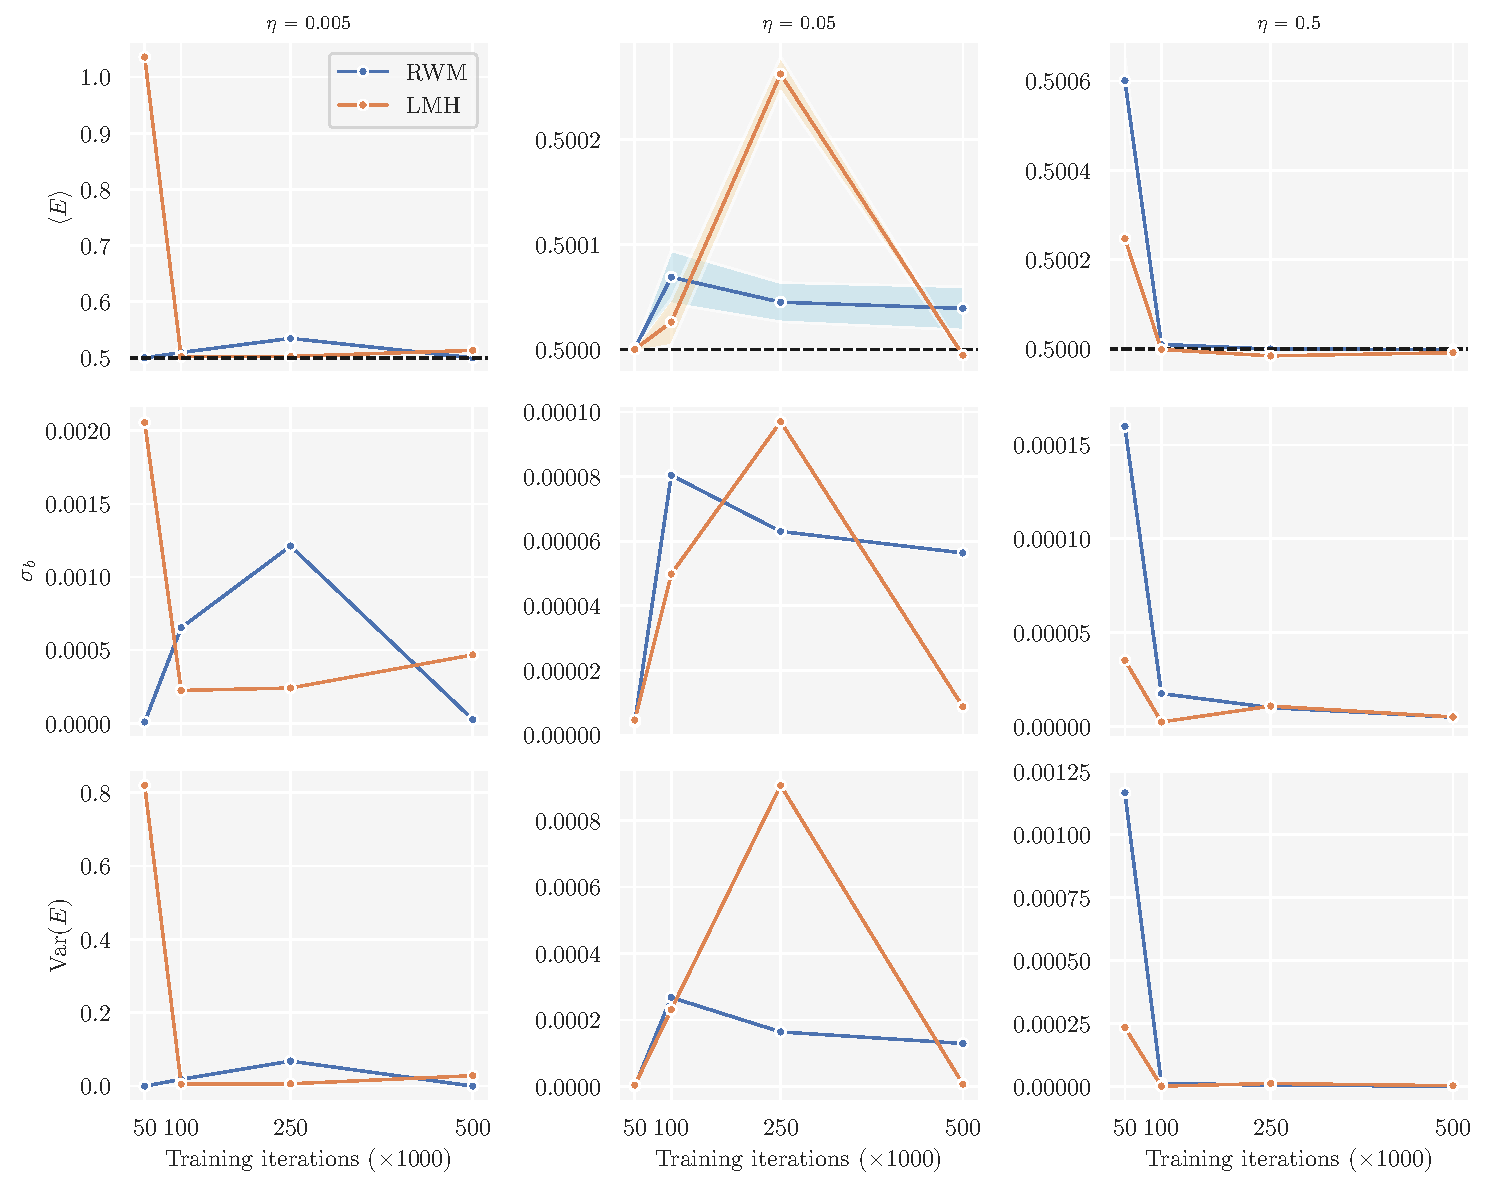
\includegraphics[width=\textwidth]{latex/figures/training_cycles_lr_batch1000.pdf}
\end{center}
\caption{The effect of the learning rate $\eta$, with the different values stated in each column's title, and the number of training iterations.   The solid lines indicates the average expected value over the $8$ chains, while the shaded region denotes the standard error of the mean. The blue lines and regions display the results from the RWM algorithm, while the orange lines show the corresponding results from the LMH algorithm.
}
\label{fig:train_iter_lr_batch1000}
\end{figure}

\autoref{fig:train_iter_lr_batch5000} is similar to the preceding figure, only here the update of parameters are done in batches of $5\,000$ training iterations. The rationale behind using a larger batch size is that the expectation values are then estimated from a larger sample size, thus increasing the accuracy of the estimate.

\begin{figure}[!htb]
\begin{center}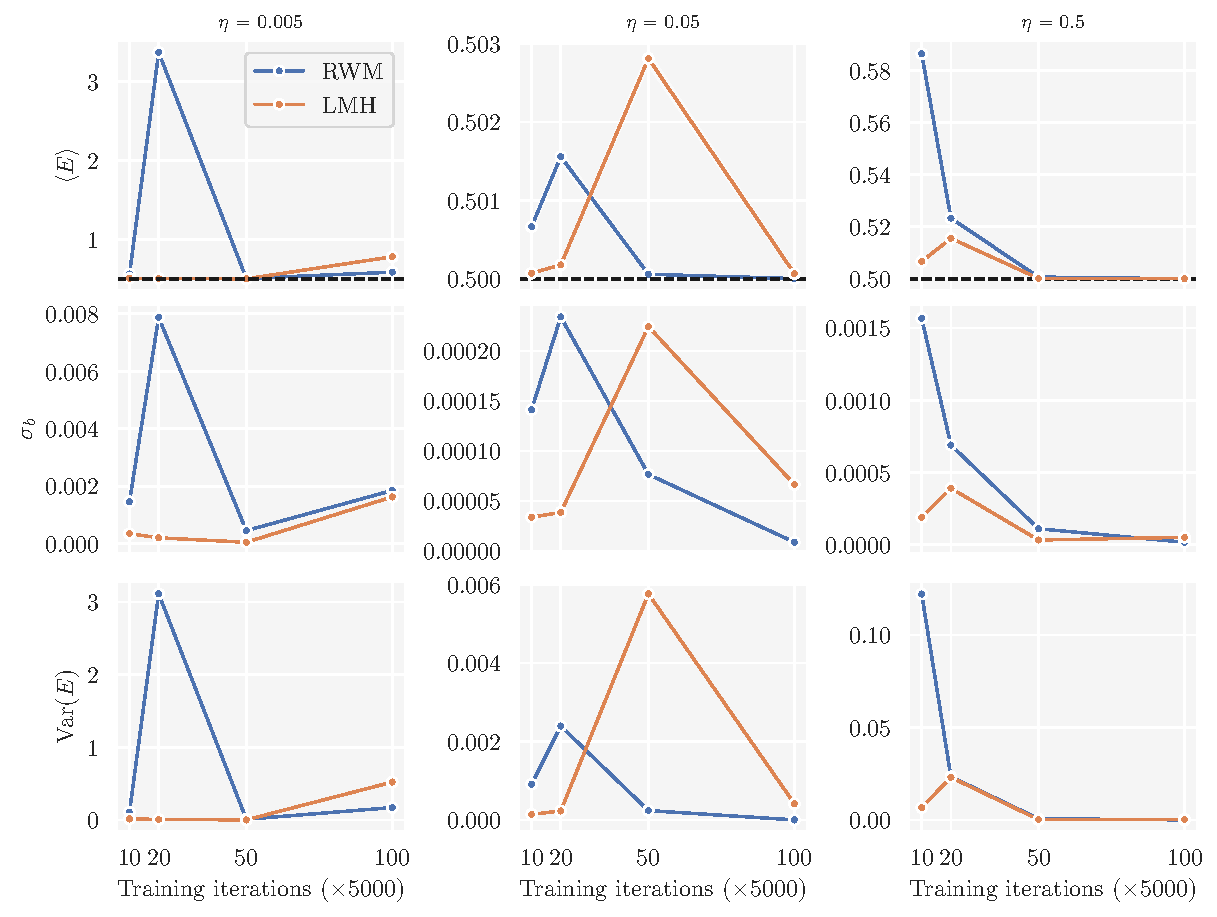
\includegraphics[width=\textwidth]{latex/figures/training_cycles_lr.pdf}
\end{center}
\caption{The effect of the learning rate $\eta$, with the different values stated in each column's title, and the number of training iterations. See the description in \autoref{fig:train_iter_lr_batch1000} for more details.}
\label{fig:train_iter_lr_batch5000}
\end{figure}

\FloatBarrier

%----------------------------------------------------------------
\subsubsection*{The Number of Hidden Neurons}
%----------------------------------------------------------------


\autoref{fig:hidden_neurons_batch_size_extra} displays comparisons of RMBs with different number of hidden neurons, $N_{\mathrm{hidden}}= \qty{1, 2, 3, 4}$, with their calculated energies (upper plots) where the left one is calculated with a batch size of $1,000$ cycles, and the right calculated with a batch size of $5,000$ cycles. The bottom plots shows the corresponding variance in the energy. The optimal number of hidden neurons for the single one-dimensional quantum dot is $2$, where the lowest error for both batch-sizes is. 

\begin{figure}[!htb]
\begin{center}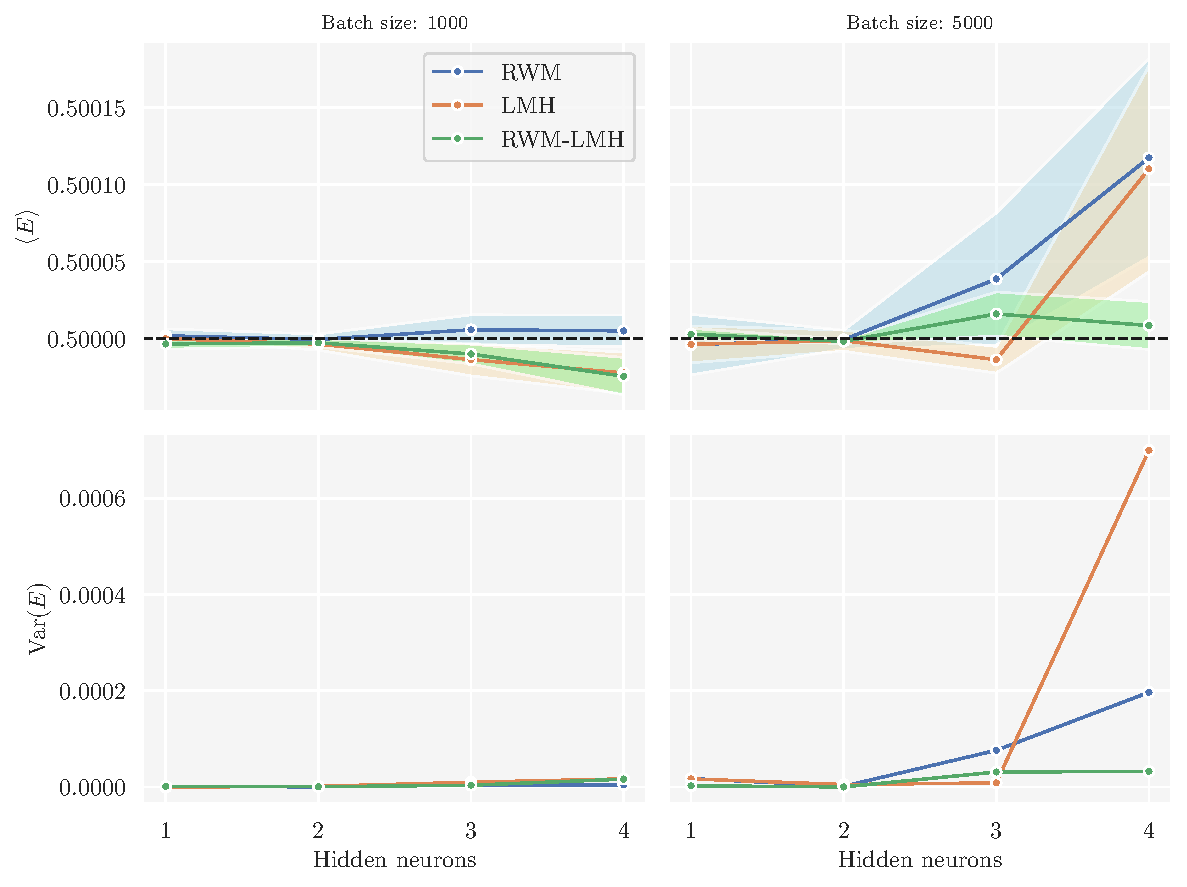
\includegraphics[width=\textwidth]{latex/figures/hidden_neurons_batch_size_extra.pdf}
\end{center}
\caption{c}
\label{fig:hidden_neurons_batch_size_extra}
\end{figure}

\FloatBarrier

%----------------------------------------------------------------
\subsubsection*{Comparing Closed-Form Gradients and Automatic Differentiation}
%----------------------------------------------------------------

\autoref{fig:runtimes} compares the runtimes of as a function of training iterations for the RWM and LMH algorithms, where calculations are performed using closed-form expressions and an automatic differentiation implementation using JAX \citep{jax2018github}. The difference in the implementations using the closed-form expressions are small, but the RWM algorithm is, as expected, due to fewer calculations in the proposal steps and acceptance probability, a little faster. When comparing with the implementations using autodifferentiation, we observe that the RWM algorithm is approximately a factor of $2$ faster on closed-form, and the LMH algorithm is approximately a factor of $3$ faster on closed-form. 

\begin{figure}[!htb]
\begin{center}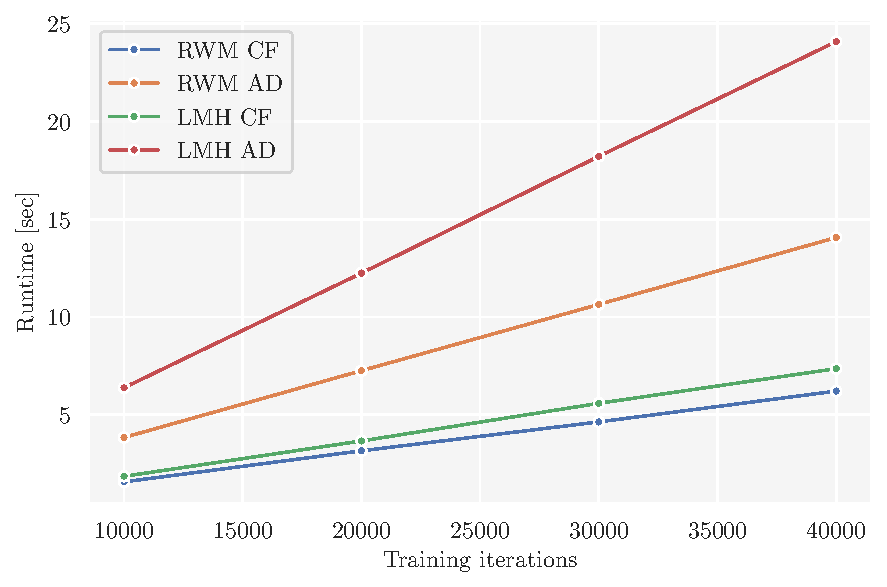
\includegraphics[scale=0.8]{latex/figures/runtimes.pdf}
\end{center}
\caption{c}
\label{fig:runtimes}
\end{figure}

\FloatBarrier

%----------------------------------------------------------------
\subsection{Interacting Quantum Dots}
%----------------------------------------------------------------

\autoref{fig:interacting_eta} displays the computed expectation values of the ground state energy against the number of hidden neurons for the two-dimensional system of two interacting quantum dots, for three different learning rates, $\eta\in\qty{0.01, 0.05, 0.5}$ using the RWM sampling algorithm. The optimal values for the learning rate and the number of hidden nodes are $\eta^{*}=0.05$ and with $6$ hidden neurons. For these hyper parameters the calculated ground state energy is found to be $E_0 = 3.059\pm0.008$ a.u. 

\begin{figure}[!htb]
\begin{center}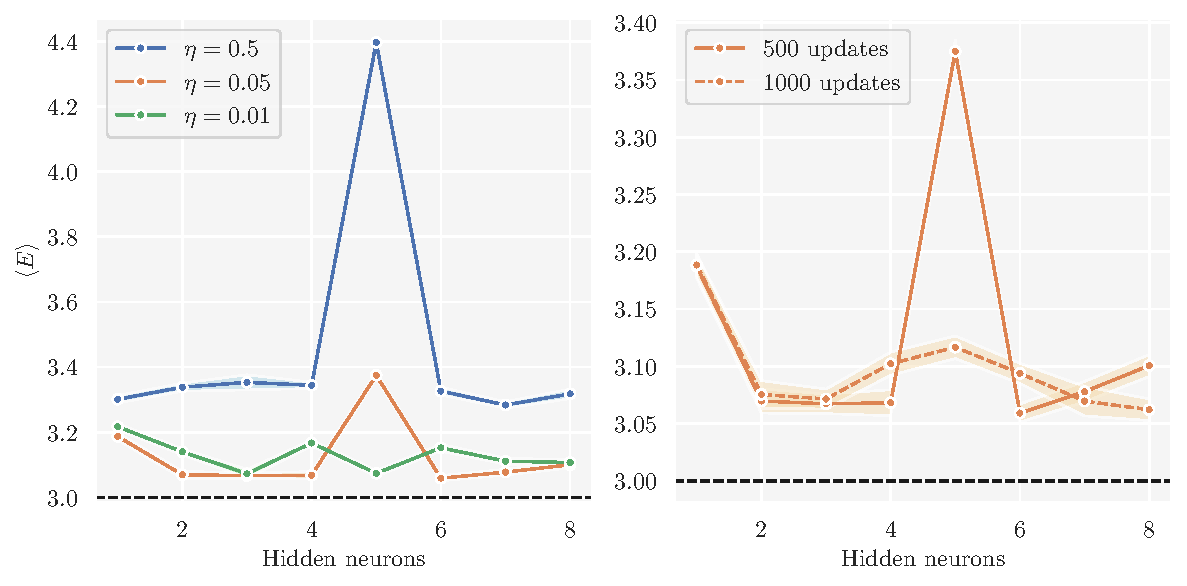
\includegraphics[width=\textwidth]{latex/figures/interacting_eta.pdf}
\end{center}
\caption{c}
\label{fig:interacting_eta}
\end{figure}

\autoref{fig:interacting_rwm_vs_lmh} shows a comparisons between the RWM and LMH sampling algorithms 

\begin{figure}[!htb]
\begin{center}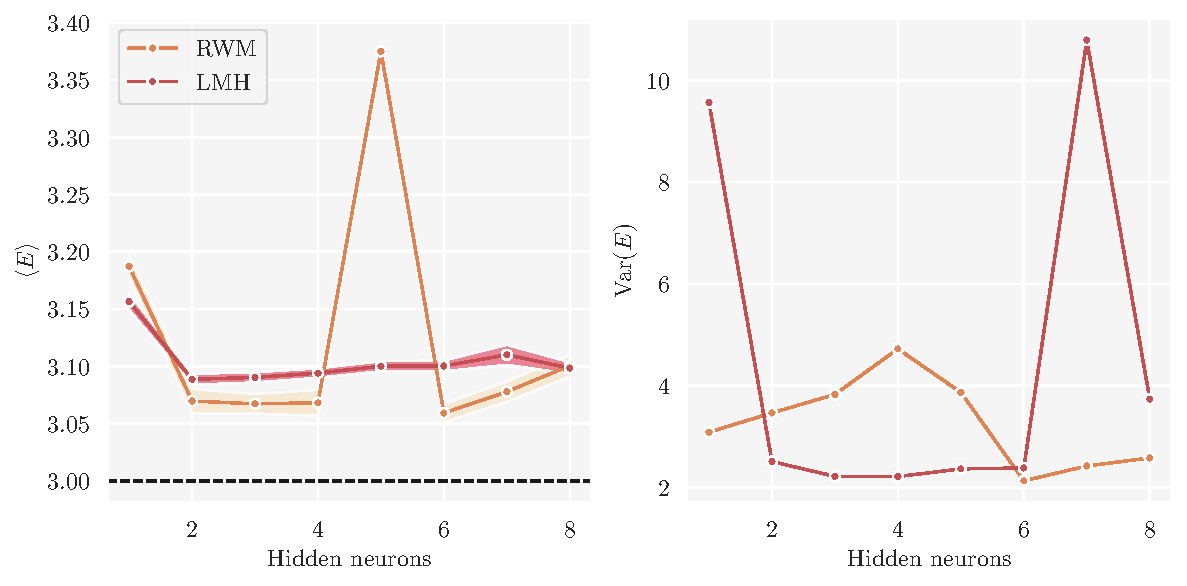
\includegraphics[width=\textwidth]{latex/figures/interacting_rwm_vs_lmh.pdf}
\end{center}
\caption{c}
\label{fig:interacting_rwm_vs_lmh}
\end{figure}










%Cost function - might be beneficial to use a cost function either based on minimizing the variance, Var(E), or on minimizing both $\langle E \rangle$ and Var(E). 

%The training itself is stochastic, and here we train the RBM parameters once, and then sample with the trained parameters with multiple Markov chains. A more rigorous approach would be to compare statistics across multiple training rounds with the same system and initial parameter settings

%Also train/optimize RBM scale